\chapter[\glsentrylong{PNI}]{\href{https://www.radiologycafe.com/frcr-physics-notes/molecular-imaging/planar-imaging/}{Planar Nuclear\\Imaging} (\gls{PNI})}
\vspace{-51ex}
\begin{flushright}
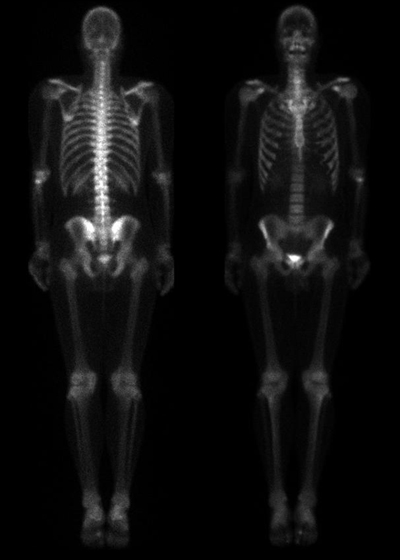
\includegraphics[width=5.5cm]{nuclearMedicineBoneScan} % https://www.hey.nhs.uk/nuclearmedicine/scanners-cameras-and-images/
\end{flushright}


\section{Acquisition}
\begin{itemize}
\item \gls{PNI} is a medical imaging technique that
  creates two-dimensional (2D) projection images of the
  three-dimensional (3D) distribution of radioactive materials within
  a patient \cite{bushberg2011essential}.
\item A radioactive isotope, incorporated into a chemical substance
  called a radiopharmaceutical, is administered to the patient
  (orally, by injection, or inhalation).
\item Once distributed according to the patient's physiological
  status, these radioisotopes \popup{emit}{For example, Technetium-99m
    (Tc-99m) emits 140-keV gamma rays, which are commonly imaged.}
  gamma rays, X-rays, or \popup{annihilation photons}{An annihilation
    photon is a type of high-energy photon produced during a unique
    interaction called annihilation, where a positron (a positively
    charged electron) combines with an electron.}.
\item Since X-rays and gamma rays are emitted isotropically (equally
  in all directions) from the radionuclide within the patient,
  \popup{collimators}{In general, an Anger scintillation camera is
    used for this.} are necessary to define the trajectory of photons
  reaching the detector and create a projection image.
\end{itemize}

\section{Clinical applications}
\begin{itemize}
\item PNI is used for functional imaging, providing insight into the
  physiological conditions (such as hyperthyroidism
  \cite{abdulla2025molecular_imaging}) rather than just the anatomy
  \cite{bushberg2011essential}.
\item Images can reveal ``hot spots'' (areas of increased
  radiopharmaceutical concentration, e.g., stress fractures or
  metastases) or ``cold spots'' (areas where normal concentration is
  altered, e.g., \popup{perfusion defects}{A perfusion defect refers
    to an area within an organ or tissue where the normal blood flow
    or distribution of a diagnostic agent is impaired or reduced. In
    medical imaging, particularly nuclear medicine, it indicates a
    functional or physiological abnormality, such as infarction
    (tissue death due to lack of blood supply) or ischemia (reduced
    blood flow), rather than a purely anatomical one.}).
\end{itemize}
\vspace{-1ex}
\begin{figure}[H]
  \centering
  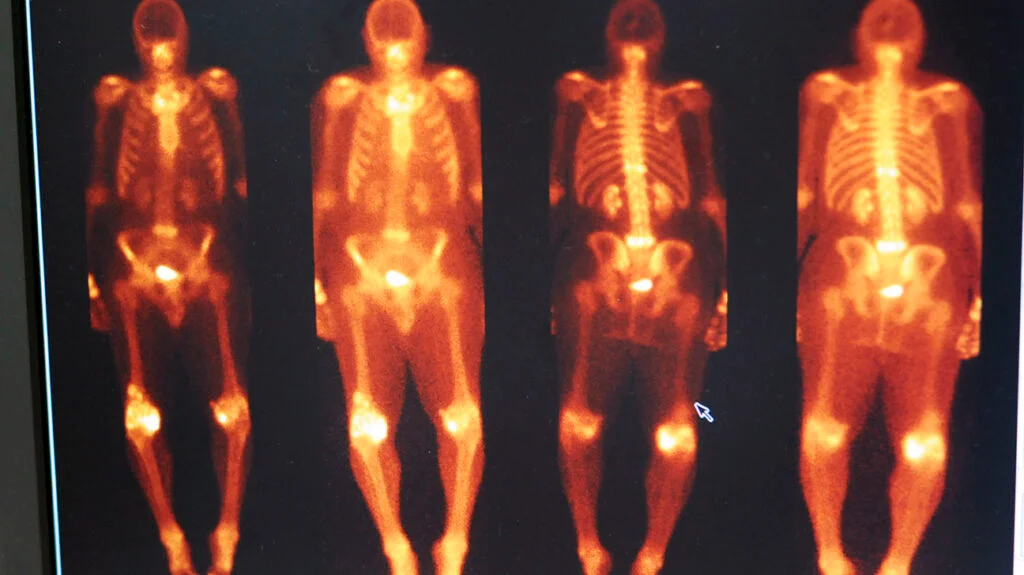
\includegraphics[width=6.5cm]{cardiac_amyloidosis}
  \caption{Hot spots showing the effects of \popup{Cardiac
      amyloidosis}{Amyloidosis occurs when the body produces amyloid
      proteins. Unlike other proteins, amyloid does not have a
      supportive role in the body. Instead, the buildup of amyloid
      protein leads to organ damage. Cardiac amyloidosis (CA) causes
      the heart to thicken and become inflexible due to abnormal
      deposits of protein in place of healthy heart tissue.}
    \cite{MNT_effects_cardiac_amyloidosis}.\label{fig:hot_spots}}
\end{figure}

\section{Quantum mottle}
\begin{itemize}
\item Due to patient safety reasons and the \popup{statistical
    nature}{Usually modeled by a Poisson distribution.} of the
  acquisition process, PNI usually generates images with a grainy
  appearance because the number of photons detected is, in most cases,
  very small.
\end{itemize}
\vspace{-1ex}
\begin{figure}[H]
  \centering
  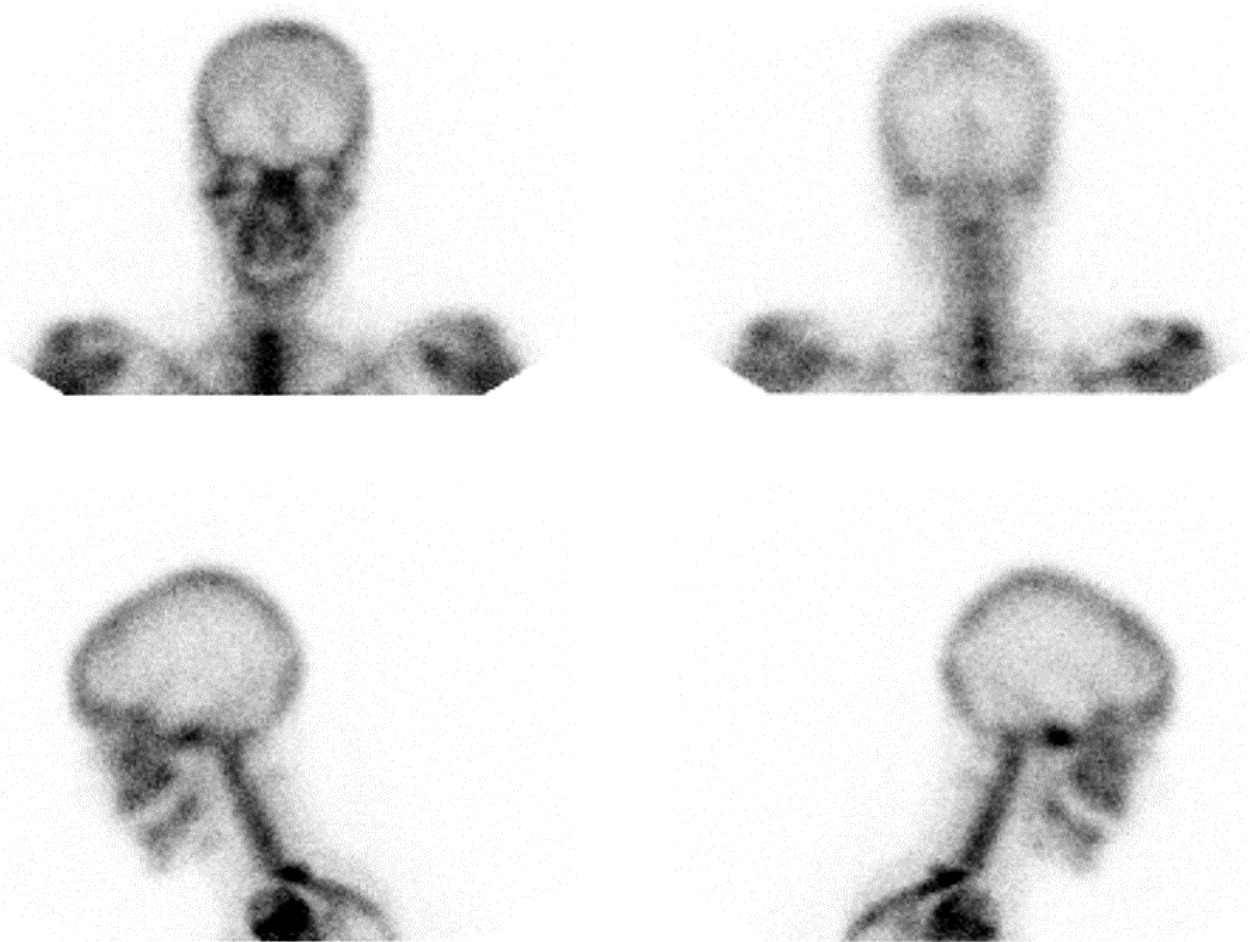
\includegraphics[width=6.5cm]{PNI_noise}
  \caption{Examples of quantum noise in \gls{PNI}
    \cite{saridin2007quantitative}.}
  \label{PNI_noise}
\end{figure}

\section{Motion blur}
\begin{itemize}
\item As a consequence of images are acquired over \popup{many seconds
    or minutes}{Basically, to gain SNR.}, it is frequent to obtain
  moved images generated by \popup{patient motion}{For example,
    respiratory motion can not be avoided.}.
\end{itemize}
\vspace{-1ex}
\begin{figure}[H]
  \centering
  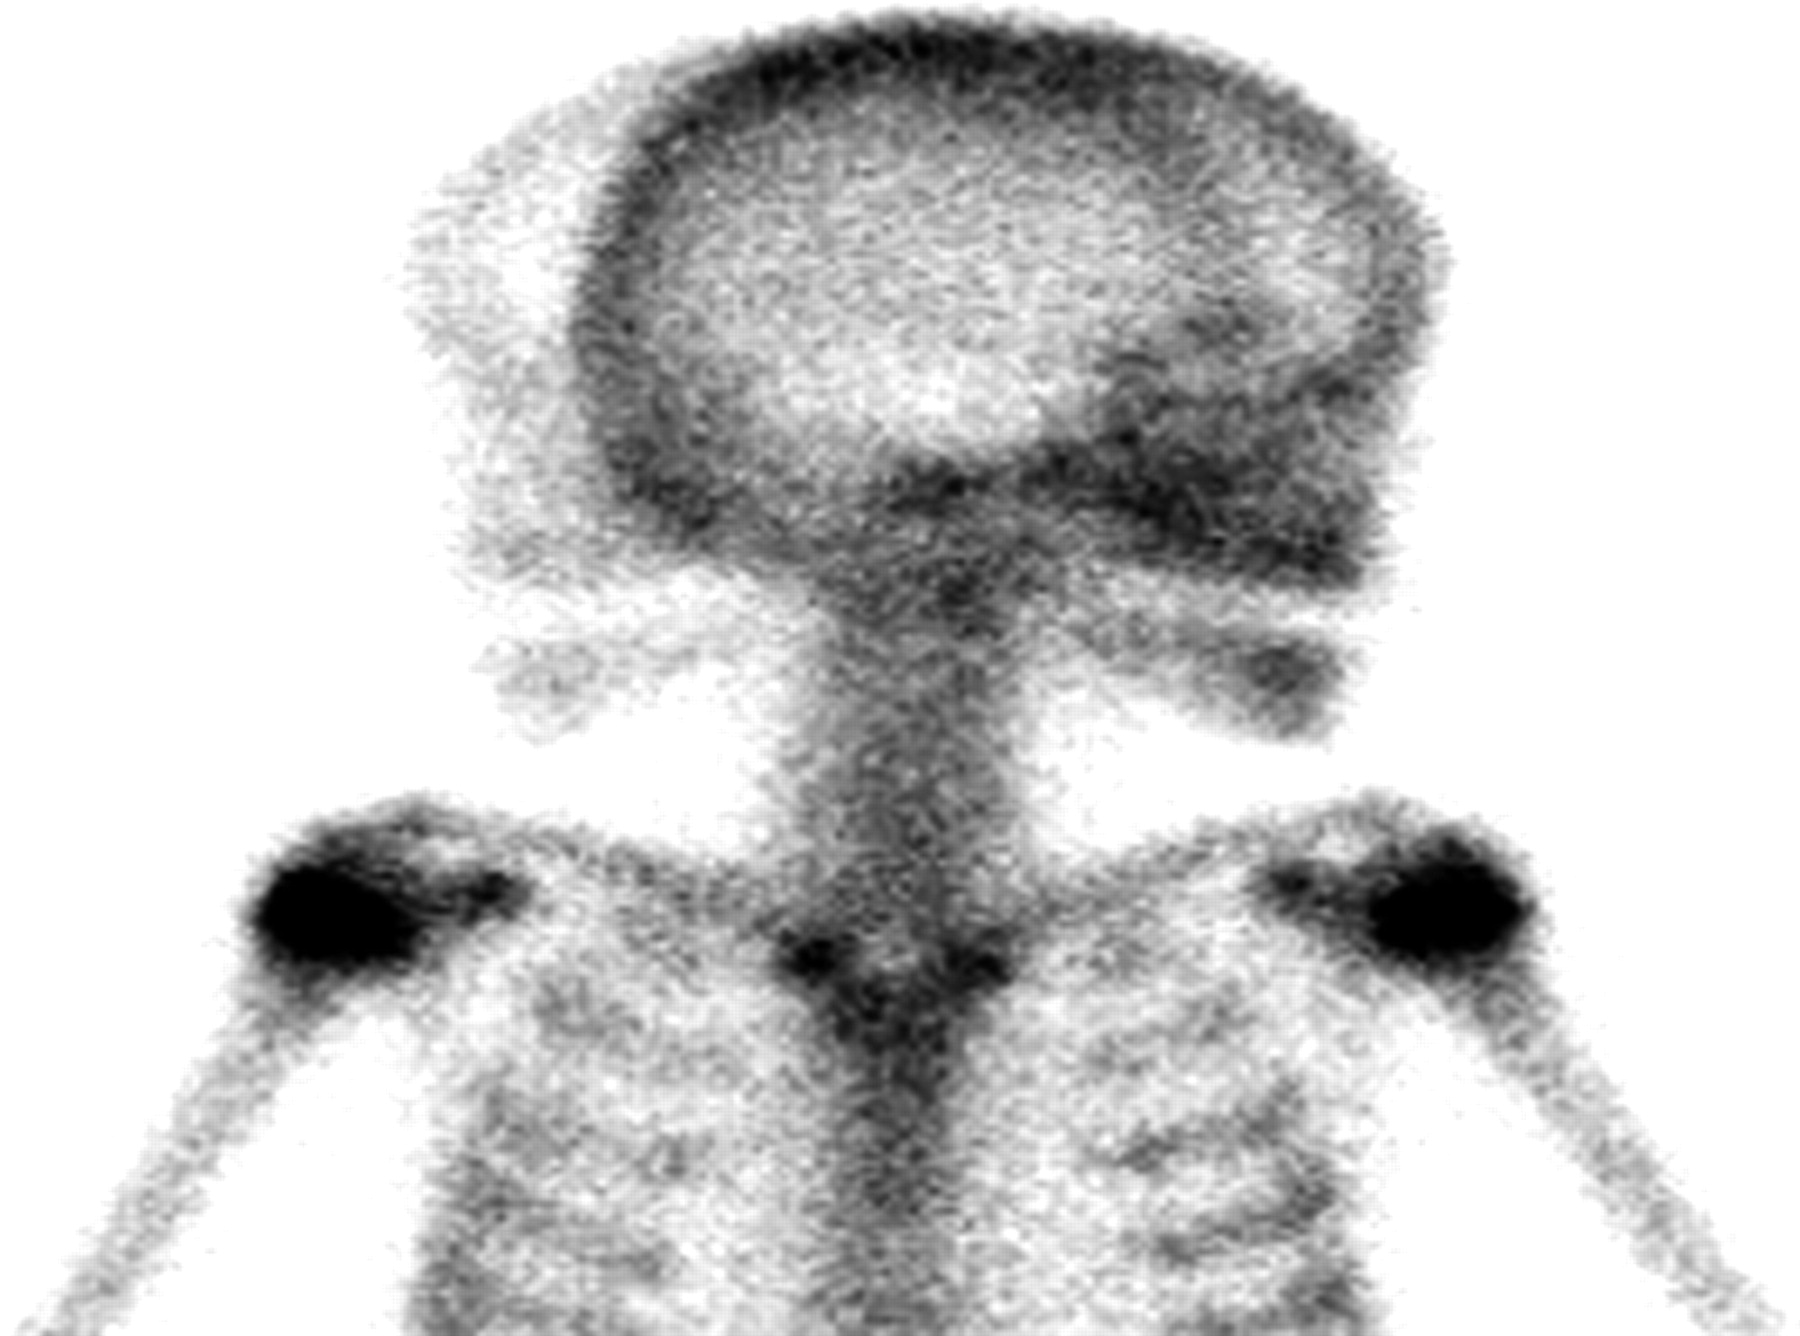
\includegraphics[width=7cm]{PNI_motion}
  \caption{Example of motion blur in \gls{PNI}
    \cite{naddaf2004technical}.}
  \label{PNI_motion}
\end{figure}
